
\documentclass[final]{beamer}
\usepackage{graphicx}
\graphicspath{ {./images/} }
\usepackage[scale=1.24]{beamerposter} % Use the beamerposter package for laying out the poster

\usetheme{confposter} % Use the confposter theme supplied with this template

\setbeamercolor{block title}{fg=ngreen,bg=white} % Colors of the block titles
\setbeamercolor{block body}{fg=black,bg=white} % Colors of the body of blocks
\setbeamercolor{block alerted title}{fg=white,bg=dblue!70} % Colors of the highlighted block titles
\setbeamercolor{block alerted body}{fg=black,bg=dblue!10} % Colors of the body of highlighted blocks
% Many more colors are available for use in beamerthemeconfposter.sty

%-----------------------------------------------------------
% Define the column widths and overall poster size
% To set effective sepwid, onecolwid and twocolwid values, first choose how many columns you want and how much separation you want between columns
% In this template, the separation width chosen is 0.024 of the paper width and a 4-column layout
% onecolwid should therefore be (1-(# of columns+1)*sepwid)/# of columns e.g. (1-(4+1)*0.024)/4 = 0.22
% Set twocolwid to be (2*onecolwid)+sepwid = 0.464
% Set threecolwid to be (3*onecolwid)+2*sepwid = 0.708

\newlength{\sepwid}
\newlength{\onecolwid}
\newlength{\twocolwid}
\newlength{\threecolwid}
\setlength{\paperwidth}{48in} % A0 width: 46.8in
\setlength{\paperheight}{36in} % A0 height: 33.1in
\setlength{\sepwid}{0.024\paperwidth} % Separation width (white space) between columns
\setlength{\onecolwid}{0.22\paperwidth} % Width of one column
\setlength{\twocolwid}{0.464\paperwidth} % Width of two columns
\setlength{\threecolwid}{0.708\paperwidth} % Width of three columns
\setlength{\topmargin}{-0.5in} % Reduce the top margin size
%-----------------------------------------------------------

\usepackage{graphicx}  % Required for including images

\usepackage{booktabs} % Top and bottom rules for tables

%----------------------------------------------------------------------------------------
%	TITLE SECTION 
%----------------------------------------------------------------------------------------

\title{\textit{Think Intensively To Think Critically.}} % Poster title

\author{Name : Basant Gera*  ,  Student ID : 40082433 , GitHub URL : \url{https://github.com/basantiscits/SOEN\_6011}, Function Assigned : Standard Deviation , Function Assigned Problem 5 :F1: arccos x , Function Assigned Problem 7 : F2: tan x} % Author(s)

\institute{Submitted to Pankaj Kamthan*} % Institution(s)

%----------------------------------------------------------------------------------------

\begin{document}

\addtobeamertemplate{block end}{}{\vspace*{2ex}} % White space under blocks
\addtobeamertemplate{block alerted end}{}{\vspace*{2ex}} % White space under highlighted (alert) blocks

\setlength{\belowcaptionskip}{2ex} % White space under figures
\setlength\belowdisplayshortskip{2ex} % White space under equations

\begin{frame}[t] % The whole poster is enclosed in one beamer frame

\begin{columns}[t] % The whole poster consists of three major columns, the second of which is split into two columns twice - the [t] option aligns each column's content to the top

\begin{column}{\sepwid}\end{column} % Empty spacer column

\begin{column}{\onecolwid} % The first column

%----------------------------------------------------------------------------------------
%	OBJECTIVES
%----------------------------------------------------------------------------------------

\begin{alertblock}{Objectives}
Objectives for the poster:
\begin{itemize}
\item Critical decisions made during the project and why those decisions were critical (Based on function assigned to me).
\item Lesson learnt by doing the project for which function assigned to me $\sigma$ \textbf{\textit{Standard Deviation}}.
\item Lesson learnt by doing the review of function assigned to me in problem 5  \textbf{\textit{ F1: arccos x}} and problem 7  \textbf{\textit{F2: tan x}}..
\item Lesson Learnt from Others.
\item Tool Used for SEP.
\end{itemize}
\end{alertblock}

%----------------------------------------------------------------------------------------
%	QUICK REVISION
%----------------------------------------------------------------------------------------

\begin{block}{Critical decisions made during the project and why those decisions were critical}
\textbf{Important decision taken are as follows : (Based on function assigned to me)}
\begin{itemize}
\item  \textit{\textbf{Done Research on Standard deviation and choosing the right formulas :}}
The Standard Deviation is a measure of how spread out numbers are. It is symbol ${\sigma}$  the Greek letter sigma.The formula is easy and is square root of variance.The standard deviation is a statistic that measures the dispersion of a data set relative to its mean. It is calculated as the square root of variance by determining the variation between each data point relative to the mean.
Here are 2 formulas which we have used over to make calculator which are as follows :
\end{itemize}

\textbf{ Population Standard Deviation}\newline
 \begin{equation*}=
    \quad \sigma  \sqrt\frac{{\Sigma (x- \overline{x})^2}}{n}
  \end{equation*}
  Where n can not be Zero.
  \textbf{Sample Standard Deviation}
 \begin{equation*}=
    \quad \sigma  \sqrt\frac{{\Sigma (x- \overline{x})^2}}{n-1}
  \end{equation*}
  Where n can not be Zero or 1.
\end{block}

\end{column} % End of the first column

\begin{column}{\sepwid}\end{column} % Empty spacer column

\begin{column}{\twocolwid} % Begin a column which is two columns wide (column 2)

\begin{columns}[t,totalwidth=\twocolwid] % Split up the two columns wide column

\begin{column}{\onecolwid}\vspace{-.6in} % The first column within column 2 (column 2.1)

%----------------------------------------------------------------------------------------
%	MATERIALS
%----------------------------------------------------------------------------------------

\begin{block}

\begin{itemize}
\item  \textit{\textbf{Choosing Graphical Interface over Textual Interface :}} I find graphical interface much more easy to use apart from that less error prone than textual interface.Below is the image of the calculator which I made in  java swing is as follows :
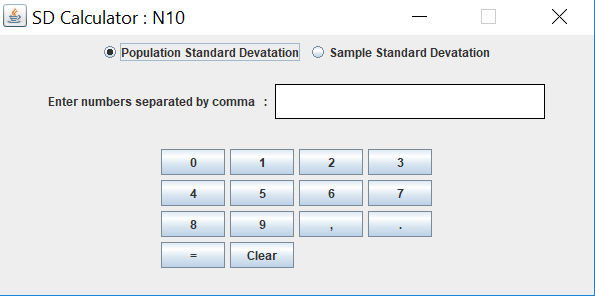
\includegraphics[scale=2.85]{Cal.PNG}\newline
\item  \textit{\textbf{Understanding not to use In-built function of Java : }} Despite of not using Java In built function tried to make own function of square root and Power to check what it takes to make it and how complex and deep enough they are.  
\end{itemize}

\end{block}

%----------------------------------------------------------------------------------------

\end{column} % End of column 2.1

\begin{column}{\onecolwid}\vspace{-.6in} % The second column within column 2 (column 2.2)

%----------------------------------------------------------------------------------------
%	P
%----------------------------------------------------------------------------------------

\begin{block}{Lesson learnt by doing the review of function assigned to me in problem 5  \textbf{\textit{ F1: arccos x}} and Problem 7  \textbf{\textit{ F2: tan x}} .}
\begin{itemize}
\item  \textit{\textbf{Learned Lambda expression}} :Lambda expression is feature of java 8.It is basically express instances of functional interfaces. for e.g $(int x)->System.out.println(2*x); $ .
\item  \textit{\textbf{Tried to debug the code in java 8 and learnt debugging in depth}} : Tried to use watch point and learnt debug in depth.
\item \textit{\textbf{Learnt to calculate how exponential is calculated wit that learn how inverse of cos works in depth}} 
\item  \textit{\textbf{Learnt Code review Strategies from req. to end}} :Learnt how to review code in JUnit too .
\item  \textit{\textbf{Learnt chekstyle and use of formatter }} :Learnt how google java style works on eclipse .
\item \textit{\textbf{Learnt how to calculate tan in java }} Learnt how tan works in java without using in built functions.
\end{itemize}


\end{block}

%----------------------------------------------------------------------------------------

\end{column} % End of column 2.2

\end{columns} % End of the split of column 2 - any content after this will now take up 2 columns width

%----------------------------------------------------------------------------------------
%	IMPORTANT To REMEMBER
%----------------------------------------------------------------------------------------

\begin{alertblock}{Standard Deviation Graph}
Standard deviation is a number used to tell how measurements for a group are spread out from the average (mean), or expected value. A low standard deviation means that most of the numbers are close to the average. A high standard deviation means that the numbers are more spread out.
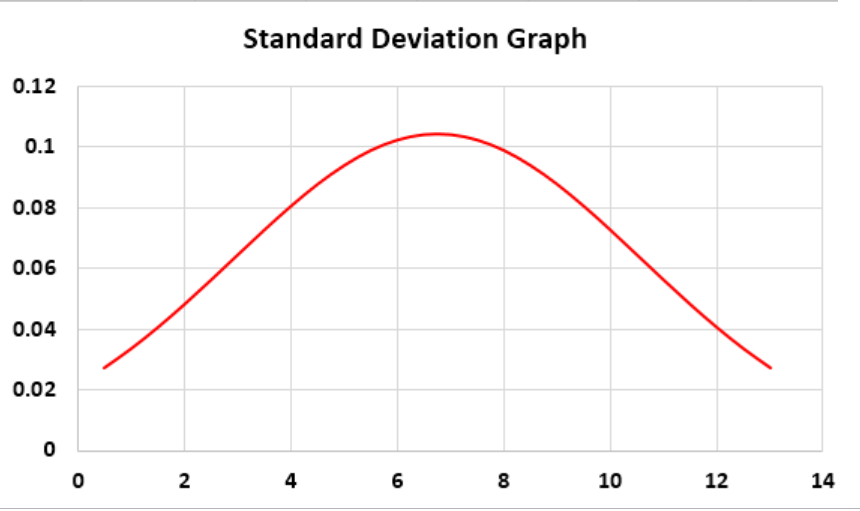
\includegraphics[scale=2.4]{SDgraph.PNG}\newline
\end{alertblock} 

%----------------------------------------------------------------------------------------

\begin{columns}[t,totalwidth=\twocolwid] % Split up the two columns wide column again



\end{columns} % End of the split of column 2

\end{column} % End of the second column

\begin{column}{\sepwid}\end{column} % Empty spacer column

\begin{column}{\onecolwid} % The third column

%----------------------------------------------------------------------------------------
%	CONCLUSION
%----------------------------------------------------------------------------------------

\begin{block}{Lesson Learnt from Others.}
\begin{itemize}
\item  \textit{\textbf{Use of java do for better understanding}} :Yes it may sound bleak but when reviewing some code is not easy task.I would not able to know what other functions is doing and try to debug it to understand what the function is trying to do .So make sure when ever you write code just write java doc on it.
\item  \textit{\textbf{Following rules and ethics which is discussed in the scrum }} : What ever discussed in team meeting is important since following that make you in sync and you would no what is write and what is wrong and what needs to be followed.
\item \textit{\textbf{Why best is required from you ?}} :You know what is best for you and how much you can handle.Never take those task which you cant address or not able to do it.Try to make your job easy and clean and do challenging work always.  
\end{itemize}
\end{block}

\begin{block}{Tools used in SEP.}
\begin{itemize}
\item  \textit{\textbf{Eclipse Neon : For Java}}  :
\includegraphics[scale=1.5]{EclipseNeon.PNG}\ 
\item  \textit{\textbf{Codacy : A review Tool}} :
\includegraphics[scale=1.5]{Codacy.PNG}\
\item  \textit{\textbf{Latex : Overleaf}} :
\includegraphics[scale=1.5]{overleaf.PNG}\ 
\item  \textit{\textbf{J Unit 4.0 : Testing}}: 
\includegraphics[scale=1.5]{Junit4.PNG}\
\end{itemize}
\end{block}


%----------------------------------------------------------------------------------------
%	ACKNOWLEDGEMENTS
%----------------------------------------------------------------------------------------

\setbeamercolor{block title}{fg=red,bg=white} % Change the block title color

\begin{block}{References.}

\begin{thebibliography}{9}
\bibitem{latexcompanion} 
\url{https://en.wikipedia.org/wiki/Standard_deviation}
 
\bibitem{einstein} 
\url{https://link.springer.com/article/10.1007/s10958-015-2539-6}

 
\bibitem{knuthwebsite} 
\url{https://sback.it/publications/icse2018seip.pdf}


\bibitem{knuthwebsite1} 
\url{https://www.ncbi.nlm.nih.gov/pmc/articles/PMC3328792/}
\end{thebibliography}



\end{block}

\setbeamercolor{block alerted title}{fg=black,bg=norange} % Change the alert block title colors
\setbeamercolor{block alerted body}{fg=black,bg=white} % Change the alert block body colors




%----------------------------------------------------------------------------------------

\end{column} % End of the third column

\end{columns} % End of all the columns in the poster

\end{frame} % End of the enclosing frame

\end{document}
